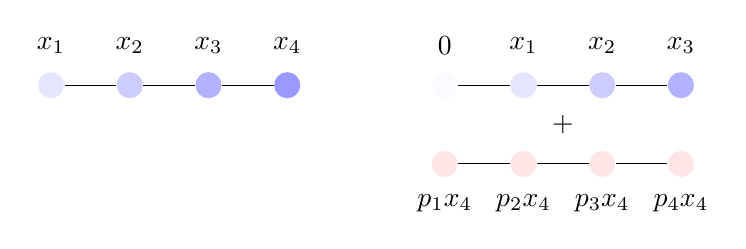
\begin{tikzpicture}[node distance=1.5cm,auto]
%%% LEFT
\node[circle, fill=blue!10] (1) at (0,0) {};
\node[circle, fill=blue!20] (2) at (1,0) {};
\node[circle, fill=blue!30] (3) at (2,0) {};
\node[circle, fill=blue!40] (4) at (3,0) {};
%
\node (11) at (0,0.5) {$x_1$};
\node (22) at (1,0.5) {$x_2$};
\node (33) at (2,0.5) {$x_3$};
\node (44) at (3,0.5) {$x_4$};
%
\draw[-] (1) to (2);
\draw[-] (2) to (3);
\draw[-] (3) to (4);
%

%%% RIGHT
\node[circle, fill=blue!2] (r1) at (5,0) {};
\node[circle, fill=blue!10] (r2) at (6,0) {};
\node[circle, fill=blue!20] (r3) at (7,0) {};
\node[circle, fill=blue!30] (r4) at (8,0) {};
%
\node (r11) at (5,0.5) {$0$};
\node (r22) at (6,0.5) {$x_1$};
\node (r33) at (7,0.5) {$x_2$};
\node (r44) at (8,0.5) {$x_3$};
%
\draw[-] (r1) to (r2);
\draw[-] (r2) to (r3);
\draw[-] (r3) to (r4);
%
%%%% BOTTOM
\node[circle, fill=red!10] (t1) at (5,-1) {};
\node[circle, fill=red!10] (t2) at (6,-1) {};
\node[circle, fill=red!10] (t3) at (7,-1) {};
\node[circle, fill=red!10] (t4) at (8,-1) {};
%
\node (t11) at (5,-1.5) {$p_1 x_4$};
\node (t22) at (6,-1.5) {$p_2 x_4$};
\node (t33) at (7,-1.5) {$p_3 x_4$};
\node (t44) at (8,-1.5) {$p_4 x_4$};
%
\draw[-] (t1) to (t2);
\draw[-] (t2) to (t3);
\draw[-] (t3) to (t4);
%
\node (p11) at (6.5,-0.5) {$+$};

%
\end{tikzpicture}